\documentclass{beamer}

\usepackage{graphicx}
\usepackage[latin1]{inputenc}
\usepackage[T1]{fontenc}
\usepackage[english]{babel}
\usepackage{listings}
\usepackage{xcolor}
\usepackage{eso-pic}
\usepackage{mathrsfs}
\usepackage{url}
\usepackage{amssymb}
\usepackage{amsmath}
\usepackage{multirow}
\usepackage{hyperref}
\usepackage{booktabs}
% \usepackage{bbm}
\usepackage{cooltooltips}
\usepackage{colordef}
\usepackage{beamerdefs}
\usepackage{lvblisting}
\usepackage{changepage}
\usepackage{xcolor}
\usepackage{graphicx}
\usepackage{epstopdf}
\usepackage{animate}

\pgfdeclareimage[height=2cm]{logobig}{hulogo}
\pgfdeclareimage[height=0.7cm]{logosmall}{Figures/small_graph.png}

\renewcommand{\titlescale}{1.0}
\renewcommand{\titlescale}{1.0}
\renewcommand{\leftcol}{0.6}


\title[XFG: Exam Presentation]{Exam Presentation: \\ Advanced methods in quantitative Finance}
\authora{Sophie Burgard}
\authorb{}
\authorc{}

\def\linka{http://lvb.wiwi.hu-berlin.de}
\def\linkb{}
\def\linkc{}

\institute{Ladislaus von Bortkiewicz Chair of Statistics \\
Humboldt--Universit�t zu Berlin \\}

\hypersetup{pdfpagemode=FullScreen}

\begin{document}

% 0-1
%%%%%%%%%%%%%%%%%%%%%%%%%%%%%%%%%%%%%%%%
\frame[plain]{

\titlepage
}

%%%%%%%%%%%%%%%%%%%%%%%%%%%%%%%%%%%%%%%%
\section{Outline}
%%%%%%%%%%%%%%%%%%%%%%%%%%%%%%%%%%%%%%%%
\useheadtemplate{
	\raisebox{-0.75cm}{\parbox{\textwidth}{
			\footnotesize{\color{isegray}
				\insertsection\ \leavevmode\leaders\hrule height3.2pt depth-2.8pt\hfill\kern0pt\ }}}}

\begin{frame}

\begin{enumerate}
\item Copula Estimation
\item Principal Component Analysis on Implied Volatility
\item Derivation: IBT Downward Nodes
\end{enumerate}

\end{frame}


\section{Copula and VaR}
\begin{frame}
\frametitle{Copula Estimation}
\begin{itemize}
\item Data: Daily data of biggest stock indices wordwide, 2005 - 2013
\end{itemize}
\begin{table}
\begin{small}

\begin{tabular}{llll}
USA: &NASDAQ & Switzerland: &SMI \\
Canada:& S$\&$P/TSX & Russia:& RTS \\
Great Britain:& FTSE100 & India: &SENSEX \\
France: &CAC40 & Japan:& NIKKEI225 \\
Germany: &DAX30 & China:& HANGSENG \\
Singapur: &STRAITS TIMES &&
\end{tabular}
\end{small}
\end{table}

\begin{itemize}
\item Procedure:
\begin{itemize}
\item Estimate Clayton and Gumbel Copula
\item Investigate tail dependency over time
\end{itemize}
\end{itemize}



\end{frame}




\begin{frame}
\frametitle{\small{Animation: Kendall's Tau based on Clayton Copula, quarterly}}
\vspace{-0.5cm}
\begin{figure}
\centering
\animategraphics[scale=0.09]{12}{PNG/clayton_}{1}{30}
\vspace{-1.7cm}
\small{\caption{Changing Kendall's Tau based on Clayton Copula}}
\end{figure}
\end{frame}

\begin{frame}
\frametitle{\small{Animation: Kendall's Tau based on Gumbel Copula, quarterly}}
\vspace{-0.5cm}
\begin{figure}
\animategraphics[scale=0.09]{12}{PNG/gumbel_}{1}{30}
\vspace{-1.7cm}
\small{\caption{Changing Kendall's Tau based on Gumbel Copula}}
\end{figure}
\end{frame}


% Use slide number after outline
\useheadtemplate{
	\raisebox{-0.75cm}{\parbox{\textwidth}{
			\footnotesize{\color{isegray}
				\insertsection\ \leavevmode\leaders\hrule height3.2pt depth-2.8pt\hfill\kern0pt\ \thesection-\thepage}}}}
\setcounter{section}{1}

\section{PCA on Implied Volatilities}
\begin{frame}
	\frametitle{Pricincipal Component Analysis on Implied Volatilities}
	\textbf{Data:} 
	\begin{itemize}
			\item VSMI: Volatility index on swiss stock market
			\item Monthly data: January 2005 until June 2016
			\item Time to maturities:
		\begin{itemize}
			\item 1-, 2-, 3 months: $\tau_{1M}$, $\tau_{2M}$, $\tau_{3M}$
			\item 1-, 2-, 3 quarter: $\tau_{1Q}$, $\tau_{2Q}$, $\tau_{3Q}$
		\end{itemize}
	\end{itemize}
\end{frame}

\begin{frame}
\frametitle{
\begin{adjustwidth}{0pt}{0pt}
\vspace{-0.9cm}
Term structure of implied volatilites
\end{adjustwidth}}
\vspace{-0.4cm}
\textbf{Background}: While "normal" volatility is a backward measure of uncertainty, implied volatility measures market expectations
\begin{figure}
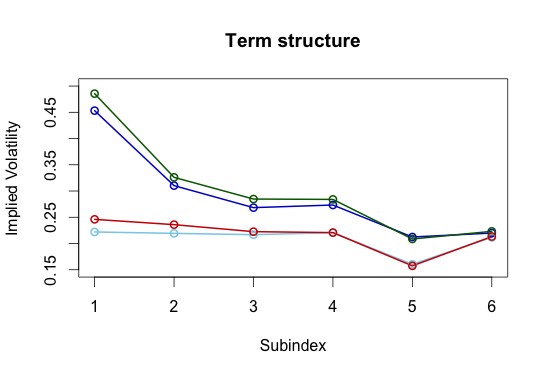
\includegraphics[scale=0.4]{Figures/termstructure.png}
\vspace{-0.8cm}
\caption{Term Structure for specific dates of VSMI: \textcolor{cyan}{15.01.2015}, \textcolor{red}{16.01.2015}, \textcolor{blue}{15.09.2008}, \textcolor{darkgreen}{16.09.2008}}
\end{figure}



\end{frame}


\begin{frame}
\frametitle{Explaining Sample Variance by PCA}
\begin{table}
\begin{tabular}{ccc}
\hline \hline
PC & Explanatory Power &  Cumulative Explanation \\
\hline
1 & 75.20 \% & 75.20 \% \\
2 & 14.92 \% & 90.12 \% \\
3 & 6.10 \% & 96.22 \% \\
4 & 2.07 \% & 98.29 \% \\ 
5 & 0.96 \% & 99.26 \% \\
6 & 0.74 \% &  100.00 \% \\  
\hline \hline
\end{tabular}
\caption{Explained sample variance using principal components}
\end{table}
\textbf{Conclusion}: First two principal components explain 90 \% of sample variance
\end{frame}

\begin{frame}
\frametitle{	
\begin{adjustwidth}{0cm}{0em}
\vspace{-0.9cm}
Effect of shocks on first and second Principal Component
\end{adjustwidth}}
\vspace{-0.5cm}
\begin{figure}
\centering
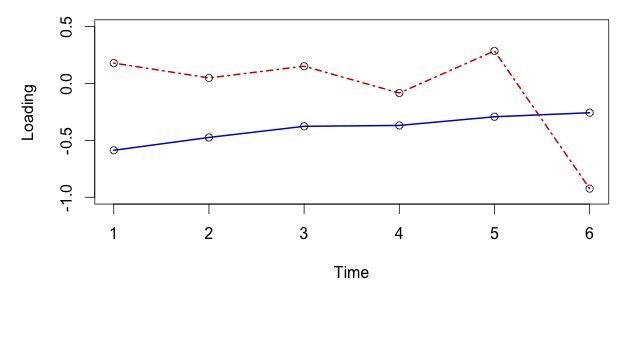
\includegraphics[scale=0.4]{Figures/factorloadings.png}
\vspace{-1.5cm}
\caption{Factor loadings for \textcolor{blue}{first} and \textcolor{red}{second} PC}
\end{figure}

\textbf{Conclusion:} 
\begin{itemize}
\item \textcolor{blue}{first} PC: similar effect for all time to maturities
\item \textcolor{red}{second} PC: strong negative effect for  $\tau_{3Q}$

\end{itemize}
\end{frame}

\section{Derivation: IBT Downward Nodes}
\begin{frame}
\frametitle{
	\begin{adjustwidth}{0pt}{0pt}
	\vspace{-0.9cm}
Implied Binomal Tree - Downward Nodes
	\end{adjustwidth}
	}
	
Risk neutral condition
\begin{align}
F^{i}_{n} = p^{n}_{i+1} S^{i+1}_{n+1}+ (1-p^{n}_{i+1}) S^{i}_{n+1}
\end{align}	
	
Arrow-Debreu prices
\begin{align*}
\lambda^{0}_{n+1}  &= e^{-r\Delta t} \left\lbrace (1 - p^{n}_{i} ) \lambda^{0}_{0} \right\rbrace \\
\lambda^{i+1}_{n+1} &= e^{-r\Delta t} \left\lbrace		\lambda^{i}_{n}	p^{n}_{i+1} +  \lambda^{i+1}_{n}	(1-p^{n}_{i+2}) \right\rbrace \\
\lambda^{n+1}_{n+1} &= e^{-r\Delta t} \left\lbrace 		\lambda^{n}_{n}	p^{n}_{i+1}	\right\rbrace \\
\end{align*}

Put option price
\begin{align}
P(K, n\Delta) = \sum_{i=0}^{n} \lambda_{n+1}^{i+1} max\left(S_{n+1}^{i+1} - K, 0 \right)
\end{align}

\end{frame}


\begin{frame}
	\begin{align*}
		 P(S, n \Delta t)\; e^{-r \Delta t}  = \; & \lambda^{0}_{n} (1-p^{n}_{1}) \, max(S -S^{0}_{n+1}) \\
									  & + \sum^{n-1}_{j=0} \left\lbrace 	\lambda^{j}_{n}	p^{n}_{j+1} +  \lambda^{j+1}_{n}	(1-p^{n}_{j+2}) 	\right\rbrace \, max(S -S^{i+1}_{n+1}) \\
									  &+ \lambda^{n}_{n}	p^{n}_{i+1} \,	 max(S -S^{n+1}_{n+1}) \\[10pt]
									  = \; & \lambda^{0}_{n} (1-p^{n}_{1}) (S -S^{0}_{n+1}) \\
									  &  + \sum^{i-1}_{j=0} \left\lbrace 	\lambda^{j}_{n}	p^{n}_{j+1} +  \lambda^{j+1}_{n}	(1-p^{n}_{j+2}) 	\right\rbrace (S -S^{i+1}_{n+1}) 							  
			\end{align*}
			
\end{frame}

\begin{frame}
\begin{small}

\begin{align*}
P(S, n \Delta t)\; e^{-r \Delta t} =\; & \textcolor{iseblue}{\lambda^{0}_{n} (1-p^{n}_{1}) \, (S -S^{0}_{n+1})}\\[5pt]
								  	   & + \textcolor{isered}{\lambda^{0}_{n} p^{n}_{1} \, (S -S^{1}_{n+1})}  +\textcolor{iseblue}{\lambda^{1}_{n} (1-p^{n}_{2}) \, (S -S^{1}_{n+1})} \\[5pt]
									   &  + \textcolor{isered}{\sum^{i-1}_{j=1} \lambda^{j}_{n}	p^{n}_{j+1} (S -S^{j+1}_{n+1})}  + \textcolor{iseblue}{\sum^{i-1}_{j=1} \lambda^{j+1}_{n}	(1-p^{n}_{j+2}) (S -S^{j+1}_{n+1})} 		\\
									   = \; &\textcolor{iseblue}{ \sum^{i}_{j=0}	 \lambda^{j}_{n} (1-p^{n}_{j+1}) (S - S^{j}_{n+1}) } + \textcolor{isered}{\sum^{i-1}_{j=0} \lambda^{j}_{n} p^{n}_{j+1} (S - S^{j+1}_{n+1})} \\													= \; & \lambda^{i}_{n}(1-p^{n}_{i+1}) (S - S^{i}_{n+1}) \\
									    & + \underbrace{\sum^{i-1}_{j=0} \lambda^{j}_{n} \left[ p^{n}_{j+1} (S - S^{j+1}_{n+1}) +  (1-p^{n}_{j+1}) (S - S^{j}_{n+1})\right] }_{= \sum^{i-1}_{j=0} \lambda^{j}_{n}(S - F^{j}_{n}) \; : = \rho_{l}}
\end{align*}

\end{small}
\end{frame}
\begin{frame}
Using option price formula:
\begin{align*}
P(s, n \Delta t) = e^{-r \Delta t} \lbrace \lambda^{i}_{n}(1-p^{n}_{i+1}) (S - S^{i}_{n+1}) + \underbrace{\sum^{i-1}_{j=0} \lambda^{j}_{n}(S - F^{j}_{n})}_{:= \rho_{l}} \rbrace
\end{align*}
and using this formula for transition probabilities, we can calculate downward nodes from risk free condition:
\begin{align*}
S^{i}_{n+1} = \frac{S^{i+1}{n+1}\left[P(S, n \Delta t) e^{r \Delta t} - \rho_{l}\right] - \lambda^{i}_{n} S(F^{i}_{n} - S^{i+1}_{n+1})}{P(S, n \Delta t) e^{r \Delta t} -\rho_{l} + \lambda^{i}_{n}(F^{i}_{n} - S^{i+1}_{n+1})}
\end{align*}
\end{frame}


\end{document}
